\subsection{Frame Synchronization : Global Summation of SOF/PLSC Detectors} 
%
Fig. \ref{fig:frame_struct} shows the Frame Structure for the communication system.
%
\begin{figure}[!ht]
\begin{center}
\includegraphics[width=\columnwidth]{./figs/frame/frame.eps}
\end{center}
\caption{Frame Structure}
\label{fig:frame_struct}
\end{figure}
Corresponding details are available in Table \ref{table:frame_struct}
\begin{table}[!ht]
\begin{center}
\input{./tables/frame_struct.tex}
\end{center}
\caption{}
\label{table:frame_struct}
\end{table}
Let the frequency offset be $\Delta f$ and phase offset be $\Delta \phi$.Then,
\begin{equation}
%\label{eq:freq_offset_model}
Y_k= X_k e^{j(2\pi\Delta fkM+\phi_k)} + V_k, \quad k = 1,\dots,N 
\end{equation}
%
assuming that no pilot symbols are trasmitted. 
Let the phase information be $\theta_k$, and defined as
%
\begin{equation}
e^{\theta(k)} = \frac{Y_k}{\abs{Y_k}}
\end{equation}
%
At the receiver, the header information is available in the form of 
\begin{align}
g_i(l)&=x_s(l)x_s(l-i), l = 0,\dots, SOF-1
\\
h_i(l)&=x_p(l)x_p(l-i), l = 0,\dots, PLSC-1
\end{align}
%
where $x_s$ are the mapped SOF symbols, $x_p$ are the scrambled PLSC  symbols, both  modulated using 8-PSK
for $i=1,2,4,8,16,32$.
The SOM is choosen as a 64-bit length such that SOF and PLS each are of 32-bit length.

A special kind of correlation is performed to obtain
\begin{align}
m_i(k)&=\sum_{l=0}^{PLSC-1} e^{j(\theta(k-l)-\theta(k-l-i))} h_i(l),
\\
n_i(k)&=\sum_{l=0}^{SOF-1} e^{j(\theta(k-l)-\theta(k-l-i))} g_i(l) ,
\\
&k = 1, \dots, N 
\end{align}
%
Compute
\begin{align}
p_i(k)=
\begin{cases}
\max \lbrak{\abs{n_i({k-PLSC})+m_i(k)},} &
\\
\rbrak{\abs{n_i({k-PLSC})-m_i(k)}} & k > PLSC
%\max \abs{m_i(k)}  & k < 64
\end{cases}
\end{align}
 GLOBAL variable $G_{R,T}(k)$  \cite{frame_offset} defined as,
\begin{equation}
G_{R,T}(k)=\sum_{i\geq1}p_i(k) , \quad i=1,2,4,8,16,32
\label{eq:global}
\end{equation}
At the receiver, let us consider we have sent two types of transmission. One is PLHEADER+DATA $\brak{Y_{k1}}$ and another is only DATA $\brak{Y_{k2}}$ and the GLOBAL variables for $\brak{Y_{k1}}$ and $\brak{Y_{k2}}$ from \eqref{eq:global} are $G1_{R,T}(k)$, $G2_{R,T}(k)$ respectively.
\subsubsection{Global Threshold Calculation}
The Global Threshold variable is defined as
\begin{align}
T&= \max \brak{ \max \brak{G1_{R,T}(k)},\max \brak{ G2_{R,T}(k)}}
\end{align} 
%\subsubsection{False Alarm Probability}
The probability of false detection of plheader when only DATA frame $\brak{Y_{k2}}$ has been sent is defined as
\begin{align}
P_{FA} &= \frac{\sum \frac{sign(\abs{Y_{k2}-T})+1}{2} }{N}
\end{align}
%\subsubsection{Missed Detection Probability}
The probability of missed detection of plheader when PLHEADER+DATA $\brak{Y_{k1}}$ has been sent is defined as
\begin{align}
P_{MD} &= \frac{\sum \frac{sign(T-\abs{Y_{k1}})+1}{2} }{N+PLSC+SOF}
\end{align}
%\subsubsection{False Alarm Probability}
%False Alarm Probability $(p_{fa})$, is the probability of false detection of plheader when only DATA frame has been sent.
%%\subsubsection{Missed Detection Probability}
%Missed Detection Probabililty $(p_{md})$, is the probability of missed detection of plheader when PLHEADER+DATA has been sent.
\subsection{Plots}
\begin{figure}[!t]
\begin{center}
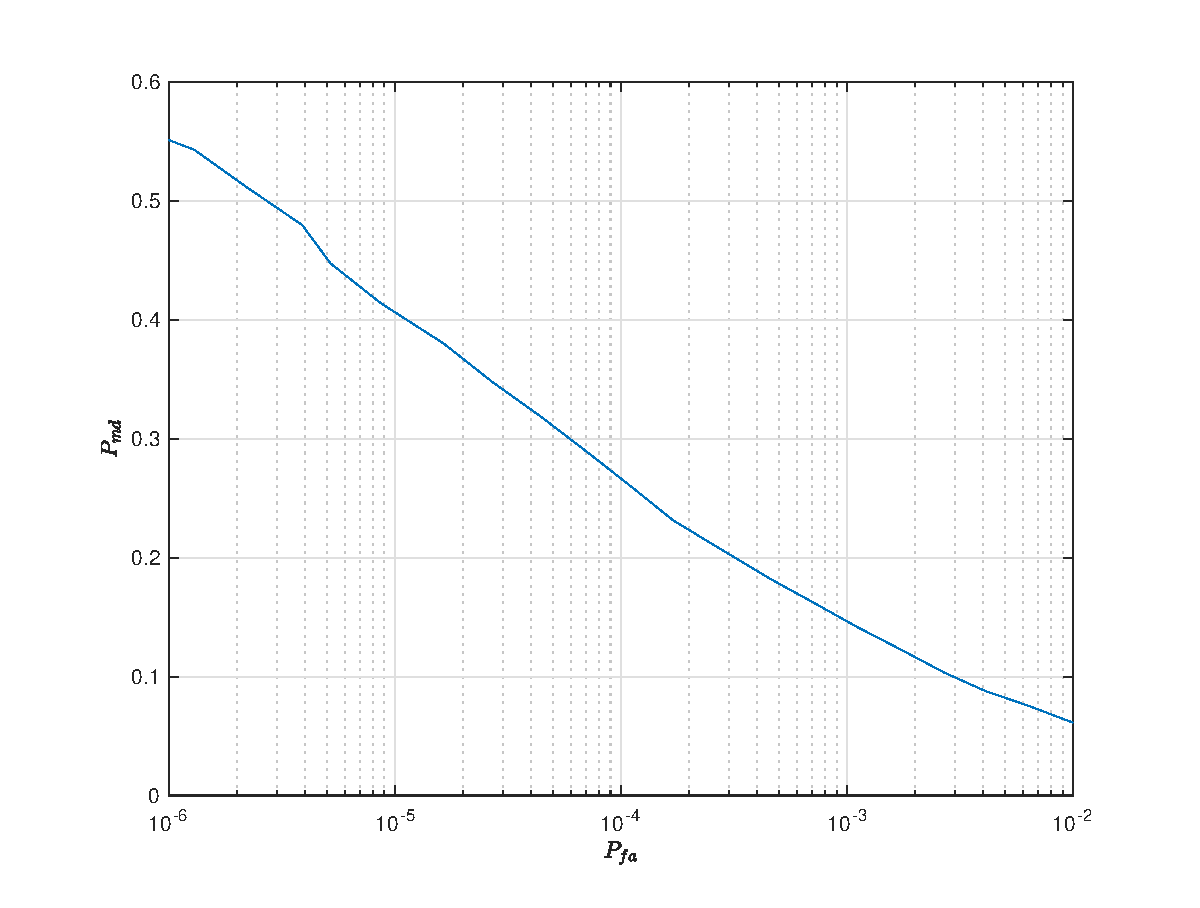
\includegraphics[width=\columnwidth]{./figs/ROC.eps}
\end{center}
\caption{Frame Synchronization Receiver Operating Characteristcs (ROC)}
\label{fig:frameoff}
\end{figure}
Fig.\ref{fig:frameoff} shows the ROC curve ($P_{FA} vs P_{MD}$)  at the receiver for frame synchronization at $\frac{E_b}{N_0}=-2$ dB and with a frequency offset of 250 KHz.

